% This is file JFM2esam.tex
% first release v1.0, 20th October 1996
%       release v1.01, 29th October 1996
%       release v1.1, 25th June 1997
%       release v2.0, 27th July 2004
%       release v3.0, 16th July 2014
%   (based on JFMsampl.tex v1.3 for LaTeX2.09)
% Copyright (C) 1996, 1997, 2014 Cambridge University Press

\documentclass{jfm}
\usepackage{graphicx}
\usepackage{epstopdf, epsfig}

\newcommand{\mrd}{\mathrm{d}}
\newcommand{\cE}{\mathcal{E}}
\newtheorem{lemma}{Lemma}
\newtheorem{corollary}{Corollary}

\shorttitle{Viscous elastic fracture}
\shortauthor{T. Large, J. Lister and D. Skinner}

\title{Viscous control of shallow elastic fracture}

\author{Tim Large\aff{1},
  John Lister\aff{2},
 \and Dominic Skinner\aff{2}}
  %\corresp{\email{jfm@damtp.cam.ac.uk}}

\affiliation{\aff{1} M.I.T., USA
\aff{2}Department of Applied Mathematics and Theoretical Physics, University of
Cambridge, UK}

\begin{document}

\maketitle

\begin{abstract}
This paper considers the problem of a semi-infinite crack parallel to the
boundary of a half plane, with the crack filled by an incompressible viscous
fluid. 
The dynamics are driven by a bending moment applied to the arm of the crack,
and we look for travelling wave solutions. We examine two models of fracture;
fracture with a single tip, and fracture with a wet tip proceded by a region
of dry fracture.
\end{abstract}

\begin{keywords}
Authors should not enter keywords on the manuscript, as these must be chosen by the 
author during the online submission process and will then be added during the 
typesetting process (see http://journals.cambridge.org/data/
\linebreak[3]relatedlink/jfm-\linebreak[3]keywords.pdf for the full list)
\end{keywords}

\section{Introduction}\label{sec:introduction}
Here we review the literature as well as describe the problem in more detail.
We have the vertical displacement $h$, the horizontal displacement $g$, the
thickness of the arm $l$, and the pressure $p$.
We look for a travelling wave solution (propagating left), with speed $c$.
%
% 
\section{Formulation of problem}\label{sec:formulation_of_problem}
%
%
\subsection{Single tip}
From lubrication, we have Poiseulle flow in the crack. We obtain
the flux, and conservation of mass as 
\begin{equation}
q = - \frac{1}{12\mu}\frac{\mrd p}{\mrd x}h^3 \, , \qquad
\frac{\partial q}{\partial x} + \frac{\partial h}{\partial t} = 0 \, ,
\end{equation}
which combined gives
\begin{equation}
\frac{\mrd p}{\mrd x} = 12\mu c / h^2 \, .
\end{equation}
Setting $p\to 0$ at $x \to \infty$, we can write this in integral form,
\begin{equation}
p(x) = -\int_x^{\infty} 12\mu c / h(\tilde{x})^2 \mrd \tilde{x} \, .
\end{equation}

From the linear theory of elasticity, due to others who have studied this 
problem, we have
\begin{equation}
\setlength{\arraycolsep}{2pt}
\left[ \begin{array}{c} 
-\sigma_y \\ -\tau_{xy}
\end{array} \right] 
= 
\left[ \begin{array}{c} 
p(x) \\ 0
\end{array} \right]
=\frac{E}{4\upi l(1-\nu^2)}  \int_0^{\infty} \mathsfbi{K} \left( 
\frac{\tilde{x}-x}{l} \right) 
\left[ \begin{array}{c} 
g'(\tilde{x}) \\ h'(\tilde{x})
\end{array} \right]
\mrd \tilde{x} \, ,
\end{equation}
%
where the integral kernel is
\begin{equation}
\setlength{\arraycolsep}{4pt}
\renewcommand{\arraystretch}{1.3}
\mathsfbi{K}(\xi) = \left[
\begin{array}{ccccc}
  K_{11}  &  K_{12}  \\
K_{21} & K_{22} \\
\end{array}  \right] 
%
= \left[
\begin{array}{ccccc}
  \frac{(32-24\xi^2)}{(\xi^2+4)^3}  &  
\frac{(48\xi^2-64)}{\xi(\xi^2+4)^3}  \\[4pt]
-\frac{(16\xi^4+16\xi^2+4)}{\xi(\xi^2+4)^3} & 
-\frac{(32 - 24\xi^2)}{(\xi^2+4)^3} 
\end{array}  \right] \, .
\end{equation}
The boundary conditions near $x=0$ are governed by fracture mechanics
\refstepcounter{equation}
$$
K_I =\lim_{x \to 0} \frac{E}{1-\nu^2} \sqrt{\frac{\upi}{8}} \sqrt{x} \, h'(x)
\, ,\qquad
K_{II} =\lim_{x \to 0} \frac{E}{1-\nu^2} \sqrt{\frac{\upi}{8}} \sqrt{x} \,
g'(x) \, .
\eqno{(\theequation{\mathit{a},\mathit{b}})}
$$
As we go to $x \gg l$, we are looking at the problem of peeling off a thin
strip from an elastic half space. We can then use beam theory approximations,
which give
\refstepcounter{equation}
$$
M(x) = \frac{El^3}{12(1-\nu^2)} \frac{\mrd^2 h}{\mrd x^2} = 
\frac{El^2}{6(1-\nu^2)} \frac{\mrd g}{\mrd x}, \qquad
p = \frac{El^3}{12(1-\nu^2)} h^{(4)}(x) 
\eqno{(\theequation{\mathit{a},\mathit{b}})}\label{eq:by-at-inf}
$$
As $x \to \infty$, $M(x) \to M$, the applied bending moment, so this gives
us boundary conditions on $h''$, $g'$.
%
\subsection{Double tip}
The equations are mostly unchanged from the single tip problem. From the
geometry of the double tip problem, a second crack tip is situated at
$x = -lL$, and $h(x),h'(x) =0$ for $x < 0$. The boundary conditions at $\infty$
are unaffected, and the boundary conditions at the crack tip become
\refstepcounter{equation}
$$
\lim_{x \to 0} \sqrt{x} \, h'(x) = L
\, ,\qquad
\lim_{x \to -Ll} \frac{E}{1-\nu^2} \sqrt{\frac{\upi}{8}} \sqrt{x} \,
g'(x) \, =K_{II} .
\eqno{(\theequation{\mathit{a},\mathit{b}})}
$$
The limits in the elasticity integral become $(-Ll,\infty)$.
%
\subsection{Rescaling}
%
We can define the following dimensionless variables
\begin{equation} 
x = l\xi,  \quad h(x) = \frac{12M(1-\nu^2)}{El}
H(\xi), \quad g(x) = \frac{12M(1-\nu^2)}{El} G(\xi) \, ,
\end{equation}
\begin{equation}
 p = \frac{3M}{\upi l^2} \Pi(\xi), \quad
K_I = Ml^{-3/2} \kappa_I, \quad
K_{II} = Ml^{-3/2} \kappa_{II}, \quad
\lambda = \frac{4\upi \mu  p^* l^3}{M^2} \, .
\end{equation}
With these scalings, the equations become
\begin{equation}
\setlength{\arraycolsep}{2pt}
\left[ \begin{array}{c} 
\Pi \\ 0
\end{array} \right]
= \int_0^{\infty} \mathsfbi{K}(\tilde{\xi} - \xi) 
\left[ \begin{array}{c} 
G'(\tilde{\xi}) \\ H'(\tilde{\xi})
\end{array} \right]
\mrd \tilde{\xi}
\end{equation}
\refstepcounter{equation}
$$
H^2 \frac{\mrd \Pi}{\mrd \xi} = \lambda
\quad \mbox{ or\ } \quad
\Pi(\xi) = -\int_{\xi}^{\infty} \lambda / H(\tilde{\xi})^2 \mrd \tilde{\xi}
%
\eqno{(\theequation{\mathit{a},\mathit{b}})}
\label{eq:govern}
$$
\begin{equation}
\lim_{\xi \to \infty} H'' = 1 , \quad \lim_{\xi \to \infty} G' = \frac{1}{2}
,\quad
\lim_{\xi \to 0} 3\sqrt{2\upi \xi} H' = \kappa_I , 
\quad
\lim_{\xi \to 0} 3\sqrt{2\upi \xi} G' = \kappa_{II} , 
\end{equation}

These shall be the governing equations for the rest of this paper.
\subsection{Beam theory asymptotics}
In the dimensionless variables, the outer asymptotics are of the form
$$
\frac{\mrd ^2 H}{\mrd \xi ^2} = \frac{1}{2}  \frac{\mrd G }{\mrd \xi},
\qquad H^{(4)}(\xi) = \frac{3}{\upi} \Pi(\xi), \qquad
\frac{\mrd ^2 H}{\mrd \xi ^2} \to 1
\eqno{(\theequation{\mathit{a},\mathit{b},\mathit{c}})}
\label{eq:outer-asymp}
$$
From integration by parts, we can write 
\begin{equation}
H''(\xi) = 1 - \frac{1}{2} \int_{\xi}^{\infty} (\tilde{\xi}-\xi)^2 H^{(5)}
(\tilde{\xi}) \mrd \tilde{\xi},
\end{equation}
provided $\lim_{\xi \to \infty} \xi H^{(3)}(\xi) = \lim_{\xi \to \infty} 
\xi^2 H^{(4)}(\xi) =0$. 
Then using equation \ref{eq:govern}a, we have that
\begin{equation}
H''(\xi) = 1 - \frac{3\lambda}{2\upi} \int_{\xi}^{\infty} 
\frac{(\tilde{\xi}-\xi)^2}{H(\tilde{\xi})^2} \mrd \tilde{\xi}.
\end{equation}
Since $H(\xi) = \frac{1}{2} \xi^2 + o(\xi^2)$, as $\xi \to \infty$, 
we can use this to get a better estimate of $H''$;
\begin{equation}
H''(\xi) = 1 - \frac{2 \lambda}{\upi} \frac{1}{\xi} + o(1/\xi).
\end{equation}
This new expression can be used to refine the error estimate from $o(1/\xi)$, to 
$O(\log(\xi)/\xi^2)$.

\subsection{Linear perturbation problem}
\emph{ This section is problably better placed elsewhere...}
The equations of the linear perturbation 
problem:
\begin{equation}
\Pi = \Pi_0 + \cE \Pi_1 + O(\cE), \quad
H = H_0 + \cE H_1 + O(\cE) \quad
\end{equation}
%
\refstepcounter{equation}
$$
\setlength{\arraycolsep}{2pt}
\left[ \begin{array}{c} 
\Pi_1 \\ 0
\end{array} \right]
= \int_0^{\infty} \mathsfbi{K}(\xi - \tilde{\xi}) 
\left[ \begin{array}{c} 
G_1'(\tilde{\xi}) \\ H_1'(\tilde{\xi})
\end{array} \right]
\mrd \tilde{\xi}, \qquad
H_0^2\Pi_1' + 2H_0 H_1 \Pi_0 ' = \lambda_1
\eqno{(\theequation{\mathit{a},\mathit{b}})}\label{eq:lin-pert}
$$
%
\refstepcounter{equation}
$$
H_1''\to 0 \mbox{ as\ } \xi \to \infty, \qquad
H_1 \sim \xi^{s} + \frac{\tilde{A}\lambda_1}{3\lambda_0^{2/3}} \xi^{2/3}
+ \dots \mbox{ as } \xi \to 0
\eqno{(\theequation{\mathit{a},\mathit{b}})}\label{eq:lin-pert-bc}
$$
But these can be made into a more convenient form, by considering instead
$\tilde{\Pi} = \Pi_0 - 3\lambda_0/\lambda_1 \Pi_1$, and similar for 
$\tilde{H}$, $\tilde{G}$. The equations become
\refstepcounter{equation}
$$
\setlength{\arraycolsep}{2pt}
\left[ \begin{array}{c} 
\tilde{\Pi} \\ 0
\end{array} \right]
= \int_0^{\infty} \mathsfbi{K}(\xi - \tilde{\xi}) 
\left[ \begin{array}{c} 
\tilde{G}'(\tilde{\xi}) \\ \tilde{H}'(\tilde{\xi})
\end{array} \right]
\mrd \tilde{\xi}, \qquad
H_0^2\tilde{\Pi}' + 2H_0 \tilde{H} \Pi_0 ' = 0
\eqno{(\theequation{\mathit{a},\mathit{b}})}\label{eq:rescaled-lin-pert}
$$
%
\refstepcounter{equation}
$$
\tilde{H}''\to 1 \mbox{ as\ } \xi \to \infty, \qquad
\tilde{H} \sim -\frac{3\lambda_0}{\lambda_1} \xi^{s} 
+ \dots \mbox{ as } \xi \to 0
\eqno{(\theequation{\mathit{a},\mathit{b}})}\label{eq:rescaled-lin-pert-bc}
$$
%
%
\section{Numerical scheme}\label{sec:numerical_scheme}
%
%%$$
\subsection{Single Tip}
We discretize the problem by taking $n+1$ points $\boldsymbol{\xi} = (\xi_0 =0,
\xi_1 \dots ,\xi_n)$ at which we measure $H'$, $G'$, and $n$ intermediate 
points $\boldsymbol{\zeta} = (\zeta_0, \dots , \zeta_{n-1})$ at which to measure
$\Pi$, so that $\xi_0 < \zeta_0 < \dots < \zeta_{n-1} < \xi_n$.
We work with $\sqrt{\xi}G'(\xi)$,
$\sqrt{\xi}H'(\xi)$ near the tip to avoid singularities.
We define $\boldsymbol{\theta}_G = [\sqrt{\xi_0}G'(\xi_0), \dots , 
\sqrt{\xi_{t-1}} G'(\xi_{t-1}), G'(\xi_t), \dots G'(\xi_n)]$,
and $\boldsymbol{\theta}_H$ similarly, as well as 
$\boldsymbol{\theta} =  [ \boldsymbol{\theta}_G, \boldsymbol{\theta}_H] $,
Typically $t \approx n/2$ was used. 
From the linearity of the elasticity integral (and the discretized 
integral) we may write 
\begin{equation}
[ \Pi(\zeta_{1}) , \dots , \Pi(\zeta_{n-1}), \, \underbrace{0 \, , \, \dots \, 
,\, 0 }_{n-1} \, ] = \mathsfbi{J} \boldsymbol{\theta} \, ,
\end{equation}
for some matrix $\mathsfbi{J}$.
One can recover $H(\xi_i)$ from $\boldsymbol{\theta}_H$. Therefore,
a discritized lubrication integral, yields an expression for 
$\Pi(\zeta_i)$ as a function of $\boldsymbol{\theta}_H$. So we can write 
\begin{equation}
[ \Pi(\zeta_{1}) , \dots , \Pi(\zeta_{n-1}), \, \underbrace{0 \, , \, \dots \, 
,\, 0 }_{n-1} \, ] = \mathsfbi{J} \boldsymbol{\theta} = \boldsymbol{f}
(\boldsymbol{\theta}_H) \, ,
\end{equation}
for some function $\boldsymbol{f}$.

Both $G'(\xi_n)$, and $H''(\xi_n)$ are known from our beam theory
asymptotic expansion. But these are linear in $\boldsymbol{\theta}$, as
$G'(\xi_n) = \theta_n$, and 
$H''(\xi_n) \approx (\theta_{2n}-\theta_{2n-1})/(\xi_n-\xi_{n-1}) $, 
Therefore we can 
add another two rows to $\mathsfbi{J}$, so that
\begin{equation}
\mathsfbi{A}\boldsymbol{\theta} = \left[ 
\boldsymbol{f}(\boldsymbol{\theta}),  
G'(\xi_n), H''(\xi_n)\right] \, .
\end{equation}
Where the $\mathsfbi{A}$ is the enlarged matrix. 
This can be solved by Newton's method from quite arbitrary initial guesses.

For $\xi_i < \xi < \xi_{i+1}$, we interpolate as
\begin{equation}
\setlength{\arraycolsep}{1pt}
G'(\xi) = \left\{ \begin{array}{l}  
\xi^{-1/2}(a_i \xi + b_i) \\[4pt]
a_i \xi + b_i
 \end{array}\right., \;\;
H'(\xi) = \left\{ \begin{array}{l}  
\xi^{-1/2}(c_i \xi^{1/2} + d_i) \\[4pt]
c_i \xi + d_i
 \end{array}\right. , \;\;
\mbox{for} \;\; \left\{ \begin{array}{l}  
i<t\\[4pt]
i\geq t
\end{array}\right.
\end{equation}
The choice of interpolating function 
was based on the appearance of the relevant functions.
We will also define $a_n,b_n,c_n,d_n$ for interpolation beyond $\xi_n$.
With this choice of interpolation,
there exist exact closed form expressions for both the lubrication integral,
and the elasticity integral, in terms of the $a_i - d_i$ coefficients.

It therefore remains to determine $a_i -d_i$ in terms of $\boldsymbol{\theta}$.
Continuity of $G'$, $H'$ imposes $2(n-1)$ linear equations. 
We also have the $2n$ equations following from the definition
of $\boldsymbol{\theta}$, (such as $a_i \xi_i + b_i = \theta_i$ for 
$t\leq i \leq n$). 

From our asymptotic expansion 
(via beam theory) we know $\theta_n = G'(\xi_n)$ and $a_n = G''(\xi_n)$. 
Therefore we can write
\begin{equation}
a_n = \frac{G''(\xi_n)}{G'(\xi_n)} \theta_n, \qquad
b_n  = \theta_n - a_n \xi_n = \left( 1 - \frac{G''(\xi_n)}
{G'(\xi_n)}\xi_n \right) \theta_n
\end{equation}
With $H$, we know that $c_n = H''(\xi_n)$, $c_{n-1} = H''(\xi_{n-1})$, and
so we have that 
\begin{equation}
c_n = \frac{H''(\xi_n)}{H''(\xi_{n-1})} c_{n-1}, \qquad
d_n = -c_n \xi_n + c_{n-1}\xi_n + d_{n-1}
\end{equation}
Therefore, we have enough equations to know the $a_i-d_i$ in terms of 
$\boldsymbol{\theta}$.

Note that we choose a value of $\lambda$, fix the boundary conditions
at $\xi \to \infty$, then solve the problem and subsequently recover
the boundary conditions at $\xi=0$ ($\kappa_I$, $\kappa_{II}$).
This can then be inverted, so that we think of $\lambda = \lambda(\kappa_I)$.
Physically, we know $\kappa_I$, and want to find $\lambda$, but in numerically
solving the problem, it makes more sense to choose $\lambda$ and recover 
$\kappa_I$.

The spacing of the points should reflect that the important 
part of the problem is happening near the tip, and this is where the points
should be concentrated. The spacing that was typically used in numerical 
calculations was 
\begin{equation}
\xi_i = \tan^2( \chi \; i/m ), \quad i=1,\dots,m < n
\end{equation}
where $\chi$ is chosen so that $\tan^2(\chi) = O(10)$, and the remaining points
are added in a geometric progression, so that 
\begin{equation}
\xi_{i+1} = (\xi_m/\xi_{m-1})\xi_{i} , \quad i = m,\dots,n-1
\end{equation}
%
%
\subsection{Linear Perturbation Problem}
%
%
From equation \ref{eq:rescaled-lin-pert-bc}b, we anticipate a 
singularity of the form $\xi^{s-1}$ in $\tilde{H}'$, (we still expect a
$\xi^{-1/2}$ singularity in $\tilde{G}'$). Therefore, the
interpolation was changed to reflect this.
Some of the integrals no longer have exact expressions. In this case, they are
calculated by a numerical integration routine.

The lubrication equation for the linear perturbation problem 
(\ref{eq:rescaled-lin-pert}b), is linear in $\tilde{H}$. Therefore, we can
obtain two expressions for $\tilde{\Pi}(\zeta_i)$ that are linear in 
$\tilde{G}'(\xi_j)$, $\tilde{H}'(\xi_j)$.
Together with the boundary conditions and beam theory asymptotics, 
(we haven't changed the integral kernel, so the asymptotics 
remain the same) there are enough equations to numerically solve the linear 
perturbation problem. There is no need to use 
Newton's method, as we can simply solve the linear set of equations.


\subsection{Double Tip}
In solving the problem of two tips situated at $-L$ and $0$, 
an additional $r$ points are taken to cover $-L \leq \xi < 0$.
The spacing of points for $\xi<0$ was chosen so that there was a concentration
of points near $-L$ and near $0$.

We interpolate $G'$ expecting a $\xi^{-1/2}$ singularity at $\xi = -L$, and
$H'$ expecting a $\xi^{-1/2}$ singularity at $\xi = 0$.
We do not 
calculate $\Pi$ for $\xi <0$ (although it is easily done), but just require that
$\sigma_{xy} = 0$ for $\xi < 0$. This provides enough equations for the problem
to be solved as before, with Newton's method. 

Note that we input $-L$ and $\lambda$ and recover $\kappa_I$, $\kappa_{II}$, where 
$\kappa_I$ is measured at $0$. Physically, for $L>0$, we must have
$\kappa_I=0$. Numerically we solve for some $\lambda$, $L$, find $\kappa_I >0$ 
and extrapolate to $\kappa_I=0$.


%
%
% 
\clearpage
\section{Results}\label{sec:Results}
%
%
%
\subsection{Single tip}
\begin{figure}
  \centerline{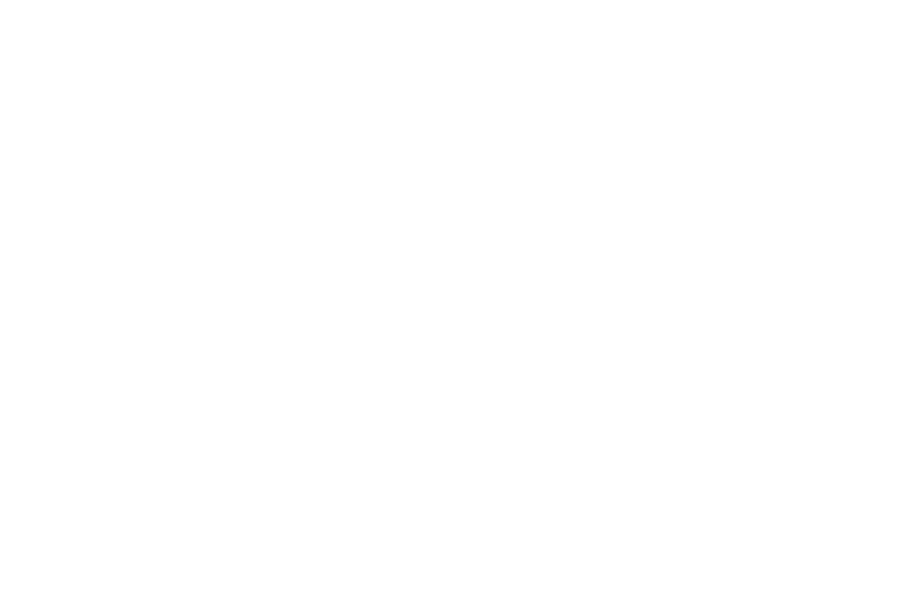
\includegraphics{./../../Graphs/hprime-p-x-full.pdf}}
  \caption{Numerical solutions for two typical values of $\kappa_I$. 
           Logarithmic scales are shown, with solid lines indicating the 
           predicted asymptotics; $H', G' \propto \xi^{-1/2}$, 
           $\Pi \propto \log(\xi)$, near $\xi=0$, 
           $H' \to \xi$, $G'\to 1/2$ as $\xi \to \infty$. 
           Figure produced with $n=465$, $\xi_n=819$.}
\end{figure}
\begin{figure}
  \centerline{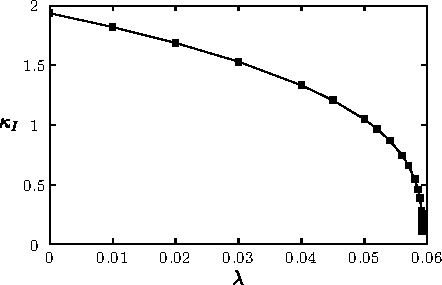
\includegraphics{./../../Graphs/K-lambda-edited.pdf}}
  \caption{Here we vary the parameter $\lambda$ and plot the change in 
           $\kappa_I$. Figure produced with $n=465$, $\xi_n = 819$.}
\end{figure}
\begin{figure}
  \centerline{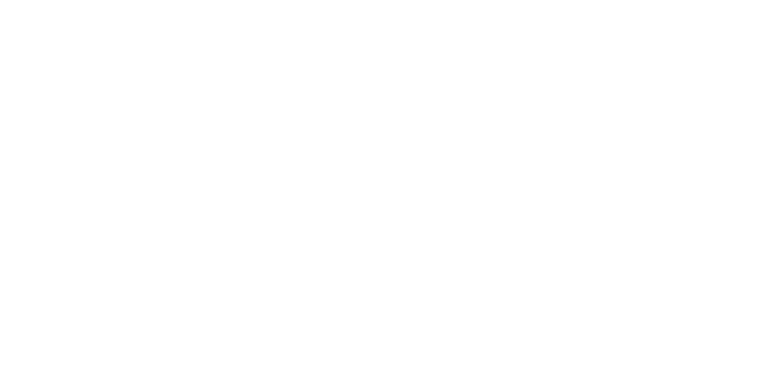
\includegraphics{./../../Graphs/hprime-x.pdf}}\label{fig:hprime-x}
  \caption{As $\kappa_I\to 0$, $H'$ moves from a $\xi^{-1/2}$ singularity
           to a $\xi^{-1/3}$ singularity. We can not calculate $\kappa_I=0$, 
           but the extrapolation to it is shown. Figure produced with $n=465$,
           $\xi_n = 819$.}
\end{figure}
\begin{figure}
  \centerline{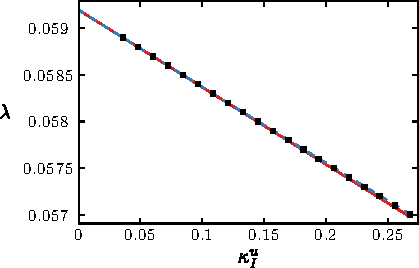
\includegraphics{./../../Graphs/l0-edited.pdf}}
  \caption{The numerical values of $\kappa_I^u$ are plotted as points against
           the values of $\lambda$. A linear fit from the two smallest $\kappa_I$ 
           values is plotted 
           as a solid line, a quadratic fit from the three smallest $\kappa_I$ 
           values is plotted as a dashed line.
           They are almost indistiguishable at this scale. 
           The difference between the two extrapolations to $\kappa_I=0$,  
           provides an estimate of the error in calculating $\lambda_0$, 
           (not accounting for the error due to $n$), which in this instance is 
           $\approx 0.002\%$. This figure was made with $n=524$, $\xi_n=846$. }
\end{figure}
\subsubsection{Calculating $H$ for $\kappa_I =0$}
$H(\xi ; \kappa_I=0)$ will be needed for the linear pertubation problem.
Numerically, for each $\xi_i$, $H'(\xi_i; \kappa_I = 0)$ is extrapolated
from $H'(\xi_i, \kappa_j)$ from two $\kappa_j$ values. Figure 
\ref{fig:hprime-x} shows that $H'(\xi; 0.21)$ 
is a good approximation to $H'(\xi;0)$, away from a boundary 
layer near $\xi=0$. The size of the boundary layer becomes smaller as $\kappa_I$
decreases, but to avoid using very small values of $\kappa_I$, the effects
of the boundary layer are removed by simply extending the linear trend present
in $0.002 < \xi < 0.003$ all the way to $\xi=0$.
\subsection{Linear perturbation problem}
We solve the linear perturbation problem. All that we really want to know
is that we see the $\tilde{H} \sim \xi^{s}$ behaviour that we expect, and we ask what the
intercept of $\tilde{H}$ is. It is perhaps worth mentioning the difficulties
in measuring the intercept and perhaps a notion of the sensitivity of the 
result on the estimate provided for $H_0$. Illustrating that is the next
figure 

\begin{figure}
 \centerline{
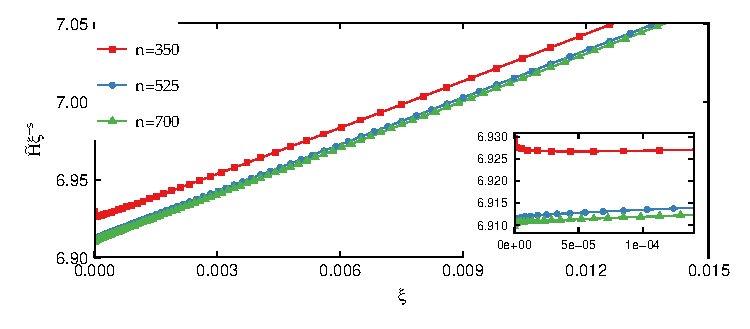
\includegraphics{./../../Graphs/linear-perturbation-plot.pdf}}
  \caption{The numerical solution of the linear perturbation problem near 
           $\xi=0$ for a selection of resolutions, all with $\xi_n = 875$. Of 
           interest, is the value of the intercept, which as shown is dependent
           on the resolution. Also shown is the numerical divergence near the 
           tip, due to the difficulty in calculating $H_0$ for $\xi \ll 1$.}
\end{figure}

\subsection{Two tips}
After the linear perturbation problem, we move on to the two tip
problem. Perhaps some graphs that show an outline of the full numerical problem
with non-zero $\kappa_I$ and $\kappa_{II}$, although these are not physical.
\begin{figure}
 \centerline{
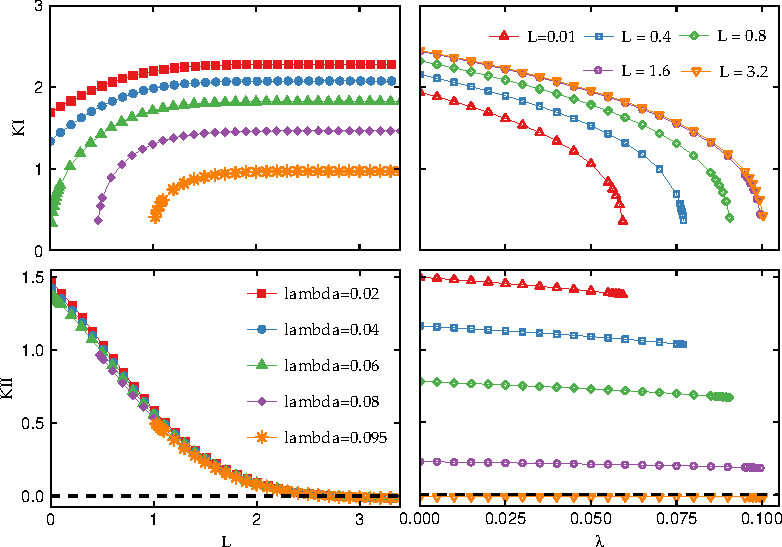
\includegraphics{./../../Graphs/KI-KII-edited.pdf}}
  \caption{Some of the numerical results for the two tip problem. Having 
           $\kappa_{I} \neq 0$ at $\xi =0$ and $L \neq 0$ is unphysical, but
           is what is found numerically. We can recover the physical solution
           by increasing $\lambda$ for fixed $L$ until $\kappa_I =0$. Figure 
           made with $n = 995$, $\xi_n = 846$.}
\end{figure}

We now move on to the $\kappa_I=0$ set of relations.
\begin{figure}
 \centerline{
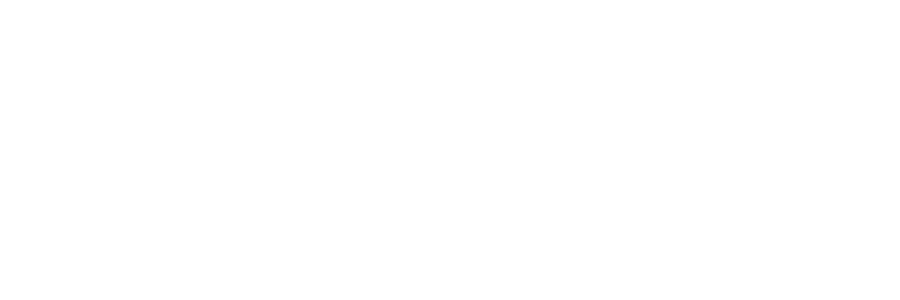
\includegraphics{./../../Graphs/KI-0.pdf}}
  \caption{The results of extrapolating to $\kappa_I = 0$. Figure 
           made with $n = 995$, $\xi_n = 846$.}
\end{figure}


\begin{figure}
 \centerline{
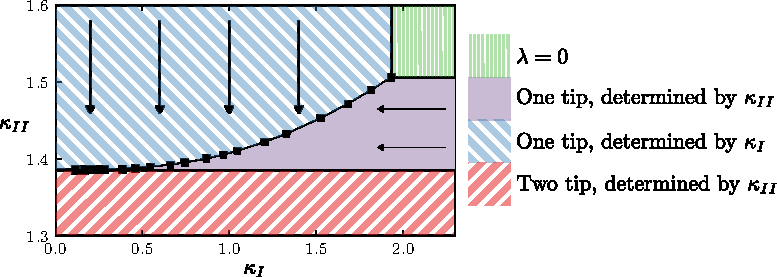
\includegraphics{./../../Graphs/catagory-edited.pdf}}
  \caption{Given values $(\kappa_I,\kappa_{II})$, this graph determines which
           frature regime occurs and so how $\lambda$ and/or $L$ should be 
           calculated. Figure made with $n=465$, $\xi_n = 819$.}
\end{figure}

\begin{figure}
 \centerline{
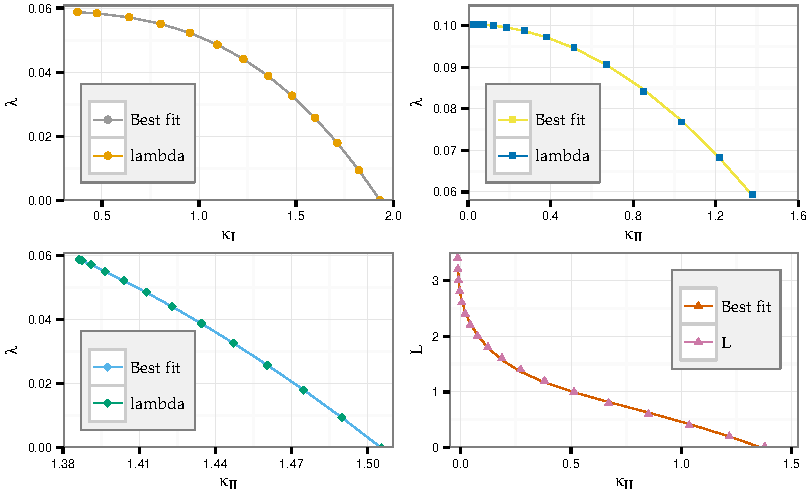
\includegraphics{./../../Graphs/overall-fit.pdf}}
  \caption{The formula valid for all $\kappa_I$. For the single tip 
           calculations, $n=815$ was used, for the double tip $n=995$. 
           $\xi_n = 846$ in both cases.  }
\end{figure}

Then we could move on to talk about the decoupling between the fluid problem
and the dry fracture problem. Relavent graphs to include would show that
$H$ really doesn't vary much with $\lambda_0$, and that given a reference
$H'$, one can construct $G'$ with relative ease.

\begin{figure}
 \centerline{
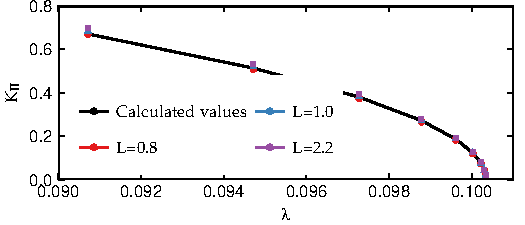
\includegraphics{./../../Graphs/fixed-fluid.pdf}}
  \caption{Reconstructing the full solution given a reference $H'$. Figure 
           made with $n=995$, $\xi_n = 846$.}
\end{figure}
\section{Discussion}

\clearpage

\begin{table}
  \begin{center}
\def~{\hphantom{0}}
  \begin{tabular}{lccc}
      $a/d$  & $M=4$   &   $M=8$ & Callan \etal \\[3pt]
       0.1   & 1.56905 & ~~1.56~ & 1.56904\\
       0.3   & 1.50484 & ~~1.504 & 1.50484\\
       0.55  & 1.39128 & ~~1.391 & 1.39131\\
       0.7   & 1.32281 & ~10.322 & 1.32288\\
       0.913 & 1.34479 & 100.351 & 1.35185\\
  \end{tabular}
  \caption{Values of $kd$ at which trapped modes occur when $\rho(\theta)=a$}
  \label{tab:kd}
  \end{center}
\end{table}

\section{Citations and references}
All papers included in the References section must be cited in the article, and vice versa. Citations should be included as, for example ``It has been shown \citep{Rogallo81} that...'' (using the {\verb}\citep} command, part of the natbib package) ``recent work by \citet{Dennis85}...'' (using {\verb}\citet}).
The natbib package can be used to generate citation variations, as shown below.\\
\verb#\citet[pp. 2-4]{Hwang70}#:\\
\citet[pp. 2-4]{Hwang70} \\
\verb#\citep[p. 6]{Worster92}#:\\
\citep[p. 6]{Worster92}\\
\verb#\citep[see][]{Koch83, Lee71, Linton92}#:\\
\citep[see][]{Koch83, Lee71, Linton92}\\
\verb#\citep[see][p. 18]{Martin80}#:\\
\citep[see][p. 18]{Martin80}\\
\verb#\citep{Brownell04,Brownell07,Ursell50,Wijngaarden68,Miller91}#:\\
\citep{Brownell04,Brownell07,Ursell50,Wijngaarden68,Miller91}\\
The References section can either be built from individual \verb#\bibitem# commands, or can be built using BibTex. The BibTex files used to generate the references in this document can be found in the zip file at http://journals.cambridge.org/\linebreak[3]data/\linebreak[3]relatedlink/\linebreak[3]jfm-ifc.zip.\\
Where there are up to ten authors, all authors' names should be given in the reference list. Where there are more than ten authors, only the first name should appear, followed by et al.\\

Acknowledgements should be included at the end of the paper, before the References section or any appendicies, and should be a separate paragraph without a heading. Several anonymous individuals are thanked for contributions to these instructions.

\appendix
\section{}\label{appA}
This appendix contains sample equations in the JFM style. Please refer to the {\LaTeX} source file for examples of how to display such equations in your manuscript.

\begin{equation}
  (\nabla^2+k^2)G_s=(\nabla^2+k^2)G_a=0
  \label{Helm}
\end{equation}

\begin{equation}
  \bnabla\bcdot\boldsymbol{v} = 0,\quad \nabla^{2}P=
    \bnabla\bcdot(\boldsymbol{v}\times \boldsymbol{w}).
\end{equation}

\begin{equation}
  G_s,G_a\sim 1 / (2\upi)\ln r
  \quad \mbox{as\ }\quad r\equiv|P-Q|\rightarrow 0,
  \label{singular}
\end{equation}

\begin{equation}
\left. \begin{array}{ll}  
\displaystyle\frac{\p G_s}{\p y}=0
  \quad \mbox{on\ }\quad y=0,\\[8pt]
\displaystyle  G_a=0
  \quad \mbox{on\ }\quad y=0,
 \end{array}\right\}
  \label{symbc}
\end{equation}


\begin{equation}
  -\frac{1}{2\upi} \int_0^{\infty} \gamma^{-1}[\mathrm exp(-k\gamma|y-\eta|)
   + \mathrm exp(-k\gamma(2d-y-\eta))] \cos k(x-\xi)t\:\mathrm{d} t,
   \qquad 0<y,\quad \eta<d,
\end{equation}

\begin{equation}
  \gamma(t) = \left\{
    \begin{array}{ll}
      -\mathrm{i}(1-t^2)^{1/2}, & t\le 1 \\[2pt]
      (t^2-1)^{1/2},         & t>1.
    \end{array} \right.
\end{equation}

\[
  -\frac{1}{2\upi}
   \pvi B(t)\frac{\cosh k\gamma(d-y)}{\gamma\sinh k\gamma d}
   \cos k(x-\xi)t\:\mathrm{d} t
\]

\begin{equation}
  G = -\frac{1}{4}\mathrm{i} (H_0(kr)+H_0(kr_1))
    - \frac{1}{\upi} \pvi\frac{\mathrm{e}^{-\kgd}}%
    {\gamma\sinh\kgd} \cosh k\gamma(d-y) \cosh k\gamma(d-\eta)
\end{equation}

Note that when equations are included in definitions, it may be suitable to render them in line, rather than in the equation environment: $\boldsymbol{n}_q=(-y^{\prime}(\theta),
x^{\prime}(\theta))/w(\theta)$.
Now $G_a=\squart Y_0(kr)+\Gat$ where
$r=\{[x(\theta)-x(\psi)]^2 + [y(\theta)-y(\psi)]^2\}^{1/2}$ and $\Gat$ is
regular as $kr\ttz$. However, any fractions displayed like this, other than $\thalf$ or $\squart$, must be written on the line, and not stacked (ie 1/3).
 
\begin{eqnarray}
  \ndq\left(\frac{1}{4} Y_0(kr)\right) & \sim &
    \frac{1}{4\upi w^3(\theta)}
    [x^{\prime\prime}(\theta)y^{\prime}(\theta)-
    y^{\prime\prime}(\theta)x^{\prime}(\theta)] \nonumber\\
  & = & \frac{1}{4\upi w^3(\theta)}
    [\rho^{\prime}(\theta)\rho^{\prime\prime}(\theta)
    - \rho^2(\theta)-2\rho^{\prime 2}(\theta)]
    \quad \mbox{as\ }\quad kr\ttz . \label{inteqpt}
\end{eqnarray}

\begin{equation}
  \frac{1}{2}\phi_i = \frac{\upi}{M} \sumjm\phi_j K_{ij}^a w_j,
  \qquad i=1,\,\ldots,\,M,
\end{equation}
where
\begin{equation}
  K_{ij}^a = \left\{
    \begin{array}{ll}
      \p G_a(\theta_i,\theta_j)/\p n_q, & i\neq j \\[2pt]
      \p\Gat(\theta_i,\theta_i)/\p n_q
      + [\rho_i^{\prime}\rho_i^{\prime\prime}-\rho_i^2-2\rho_i^{\prime 2}]
      / 4\upi w_i^3, & i=j.
  \end{array} \right.
\end{equation}


\refstepcounter{equation}
$$
  \rho_l = \lim_{\zeta \rightarrow Z^-_l(x)} \rho(x,\zeta), \quad
  \rho_{u} = \lim_{\zeta \rightarrow Z^{+}_u(x)} \rho(x,\zeta)
  \eqno{(\theequation{\mathit{a},\mathit{b}})}\label{eq35}
$$

\begin{equation}
  (\rho(x,\zeta),\phi_{\zeta\zeta}(x,\zeta))=(\rho_0,N_0)
  \quad \mbox{for}\quad Z_l(x) < \zeta < Z_u(x).
\end{equation}


\begin{subeqnarray}
  \tau_{ij} & = &
    (\overline{\overline{u}_i \overline{u}_j}
    - \overline{u}_i\overline{u}_j)
    + (\overline{\overline{u}_iu^{SGS}_j
    + u^{SGS}_i\overline{u}_j})
    + \overline{u^{SGS}_iu^{SGS}_j},\\[3pt]
  \tau^\theta_j & = &
    (\overline{\overline{u}_j\overline{\theta}}
    - \overline{u}_j \overline{\theta})
    + (\overline{\overline{u}_j\theta^{SGS}
    + u^{SGS}_j \overline{\theta}})
    + \overline{u^{SGS}_j\theta^{SGS}}.
\end{subeqnarray}

\begin{equation}
\setlength{\arraycolsep}{0pt}
\renewcommand{\arraystretch}{1.3}
\slsQ_C = \left[
\begin{array}{ccccc}
  -\omega^{-2}V'_w  &  -(\alpha^t\omega)^{-1}  &  0  &  0  &  0  \\
  \displaystyle
  \frac{\beta}{\alpha\omega^2}V'_w  &  0  &  0  &  0  &  \mathrm{i}\omega^{-1} \\
  \mathrm{i}\omega^{-1}  &  0  &  0  &  0  &  0  \\
  \displaystyle
  \mathrm{i} R^{-1}_{\delta}(\alpha^t+\omega^{-1}V''_w)  &  0
    & -(\mathrm{i}\alpha^tR_\delta)^{-1}  &  0  &  0  \\
  \displaystyle
  \frac{\mathrm{i}\beta}{\alpha\omega}R^{-1}_\delta V''_w  &  0  &  0
    &  0  & 0 \\
  (\mathrm{i}\alpha^t)^{-1}V'_w  &  (3R^{-1}_{\delta}+c^t(\mathrm{i}\alpha^t)^{-1})
    &  0  &  -(\alpha^t)^{-2}R^{-1}_{\delta}  &  0  \\
\end{array}  \right] .
\label{defQc}
\end{equation}

\begin{equation}
\etb^t = \skew2\hat{\etb}^t \exp [\mathrm{i} (\alpha^tx^t_1-\omega t)],
\end{equation}
where $\skew2\hat{\etb}^t=\boldsymbol{b}\exp (\mathrm{i}\gamma x^t_3)$. 
\begin{equation}
\mbox{Det}[\rho\omega^2\delta_{ps}-C^t_{pqrs}k^t_qk^t_r]=0,
\end{equation}

\begin{equation}
 \langle k^t_1,k^t_2,k^t_3\rangle = \langle
\alpha^t,0,\gamma\rangle  
\end{equation}

\begin{equation}
\boldsymbol{f}(\theta,\psi) = (g(\psi)\cos \theta,g(\psi) \sin \theta,f(\psi)).
\label{eq41}
\end{equation}

\begin{eqnarray}
f(\psi_1) = \frac{3b}{\upi[2(a+b \cos \psi_1)]^{{3}/{2}}}
  \int^{2\upi}_0 \frac{(\sin \psi_1 - \sin \psi)(a+b \cos \psi)^{1/2}}%
  {[1 - \cos (\psi_1 - \psi)](2+\alpha)^{1/2}}\mathrm{d}x,
\label{eq42}
\end{eqnarray}
\begin{eqnarray}
g(\psi_1) & = & \frac{3}{\upi[2(a+b \cos \psi_1)]^{{3}/{2}}}
  \int^{2\upi}_0 \left(\frac{a+b \cos \psi}{2+\alpha}\right)^{1/2}
  \left\{ \astrut f(\psi)[(\cos \psi_1 - b \beta_1)S + \beta_1P]
  \right. \nonumber\\
&& \mbox{}\times \frac{\sin \psi_1 - \sin \psi}{1-\cos(\psi_1 - \psi)}
  + g(\psi) \left[\left(2+\alpha - \frac{(\sin \psi_1 - \sin \psi)^2}
  {1- \cos (\psi - \psi_1)} - b^2 \gamma \right) S \right.\nonumber\\
&& \left.\left.\mbox{} + \left( b^2 \cos \psi_1\gamma -
  \frac{a}{b}\alpha \right) F(\frac{1}{2}\upi, \delta) - (2+\alpha)
  \cos\psi_1 E(\frac{1}{2}\upi, \delta)\right] \astrut\right\} \mathrm{d} \psi,
\label{eq43}
\end{eqnarray}
\begin{equation}
\alpha = \alpha(\psi,\psi_1) = \frac{b^2[1-\cos(\psi-\psi_1)]}%
  {(a+b\cos\psi) (a+b\cos\psi_1)},
  \quad
  \beta - \beta(\psi,\psi_1) = \frac{1-\cos(\psi-\psi_1)}{a+b\cos\psi}.
\end{equation}


\begin{equation}
\left. \begin{array}{l}
\displaystyle
H(0) = \frac{\epsilon \overline{C}_v}{\tilde{v}^{{1}/{2}}_T
(1- \beta)},\quad H'(0) = -1+\epsilon^{{2}/{3}} \overline{C}_u
+ \epsilon \skew5\hat{C}_u'; \\[16pt]
\displaystyle
H''(0) = \frac{\epsilon u^2_{\ast}}{\tilde{v}^{{1}/{2}}
_T u^2_P},\quad H' (\infty) = 0.
\end{array} \right\}
\end{equation}

\begin{lemma}
Let $f(z)$ be a trial \citet[][pp.~231--232]{Batchelor59} function defined on $[0,1]$.  Let $\varLambda_1$ denote
the ground-state eigenvalue for $-\mathrm{d}^2g/\mathrm{d} z^2=\varLambda g$,
where $g$ must satisfy $\pm\mathrm{d} g/\mathrm{d} z+\alpha g=0$ at $z=0,1$
for some non-negative constant~$\alpha$.  Then for any $f$ that is not
identically zero we have
\begin{equation}
\frac{\displaystyle
  \alpha(f^2(0)+f^2(1)) + \int_0^1 \left(
  \frac{\mathrm{d} f}{\mathrm{d} z} \right)^2 \mathrm{d} z}%
  {\displaystyle \int_0^1 f^2\mathrm{d} z}
\ge \varLambda_1 \ge
\left( \frac{-\alpha+(\alpha^2+8\upi^2\alpha)^{1/2}}{4\upi} \right)^2.
\end{equation}
\end{lemma}

\begin{corollary}
Any non-zero trial function $f$ which satisfies the boundary condition
$f(0)=f(1)=0$ always satisfies
\begin{equation}
  \int_0^1 \left( \frac{\mathrm{d} f}{\mathrm{d} z} \right)^2 \mathrm{d} z.
\end{equation}
\end{corollary}

\bibliographystyle{jfm}
% Note the spaces between the initials
\bibliography{elastic-fracture}

\end{document}
